\documentclass{article}
\usepackage[utf8]{inputenc}
\usepackage{hyperref}
\usepackage{graphicx}
\usepackage{listings}
\usepackage{xcolor}
\usepackage{geometry}
\usepackage{tikz}
\usetikzlibrary{positioning, arrows.meta, calc, backgrounds, fit, shapes}

\geometry{
    a4paper,
    total={170mm,257mm},
    left=20mm,
    top=20mm,
}

\title{Technical Summary: Voice Agent Architecture}
\author{Final Doers Team}
\date{\today}

\begin{document}

\maketitle

\section{High-Level Architecture}
The system uses a \textbf{Hybrid Client-Server Architecture} designed for ultra-low latency and secure interactions.

\begin{itemize}
    \item \textbf{Frontend (Client)}: Handles the real-time WebSocket connection to Google's Gemini Live API, audio processing (recording/playback), and session state management.
    \item \textbf{Backend (Server)}: Acts as an authorization gatekeeper and persistence layer. It does \textit{not} proxy the audio stream, ensuring zero added latency.
\end{itemize}

\begin{figure}[h]
    \centering
    \resizebox{\textwidth}{!}{
    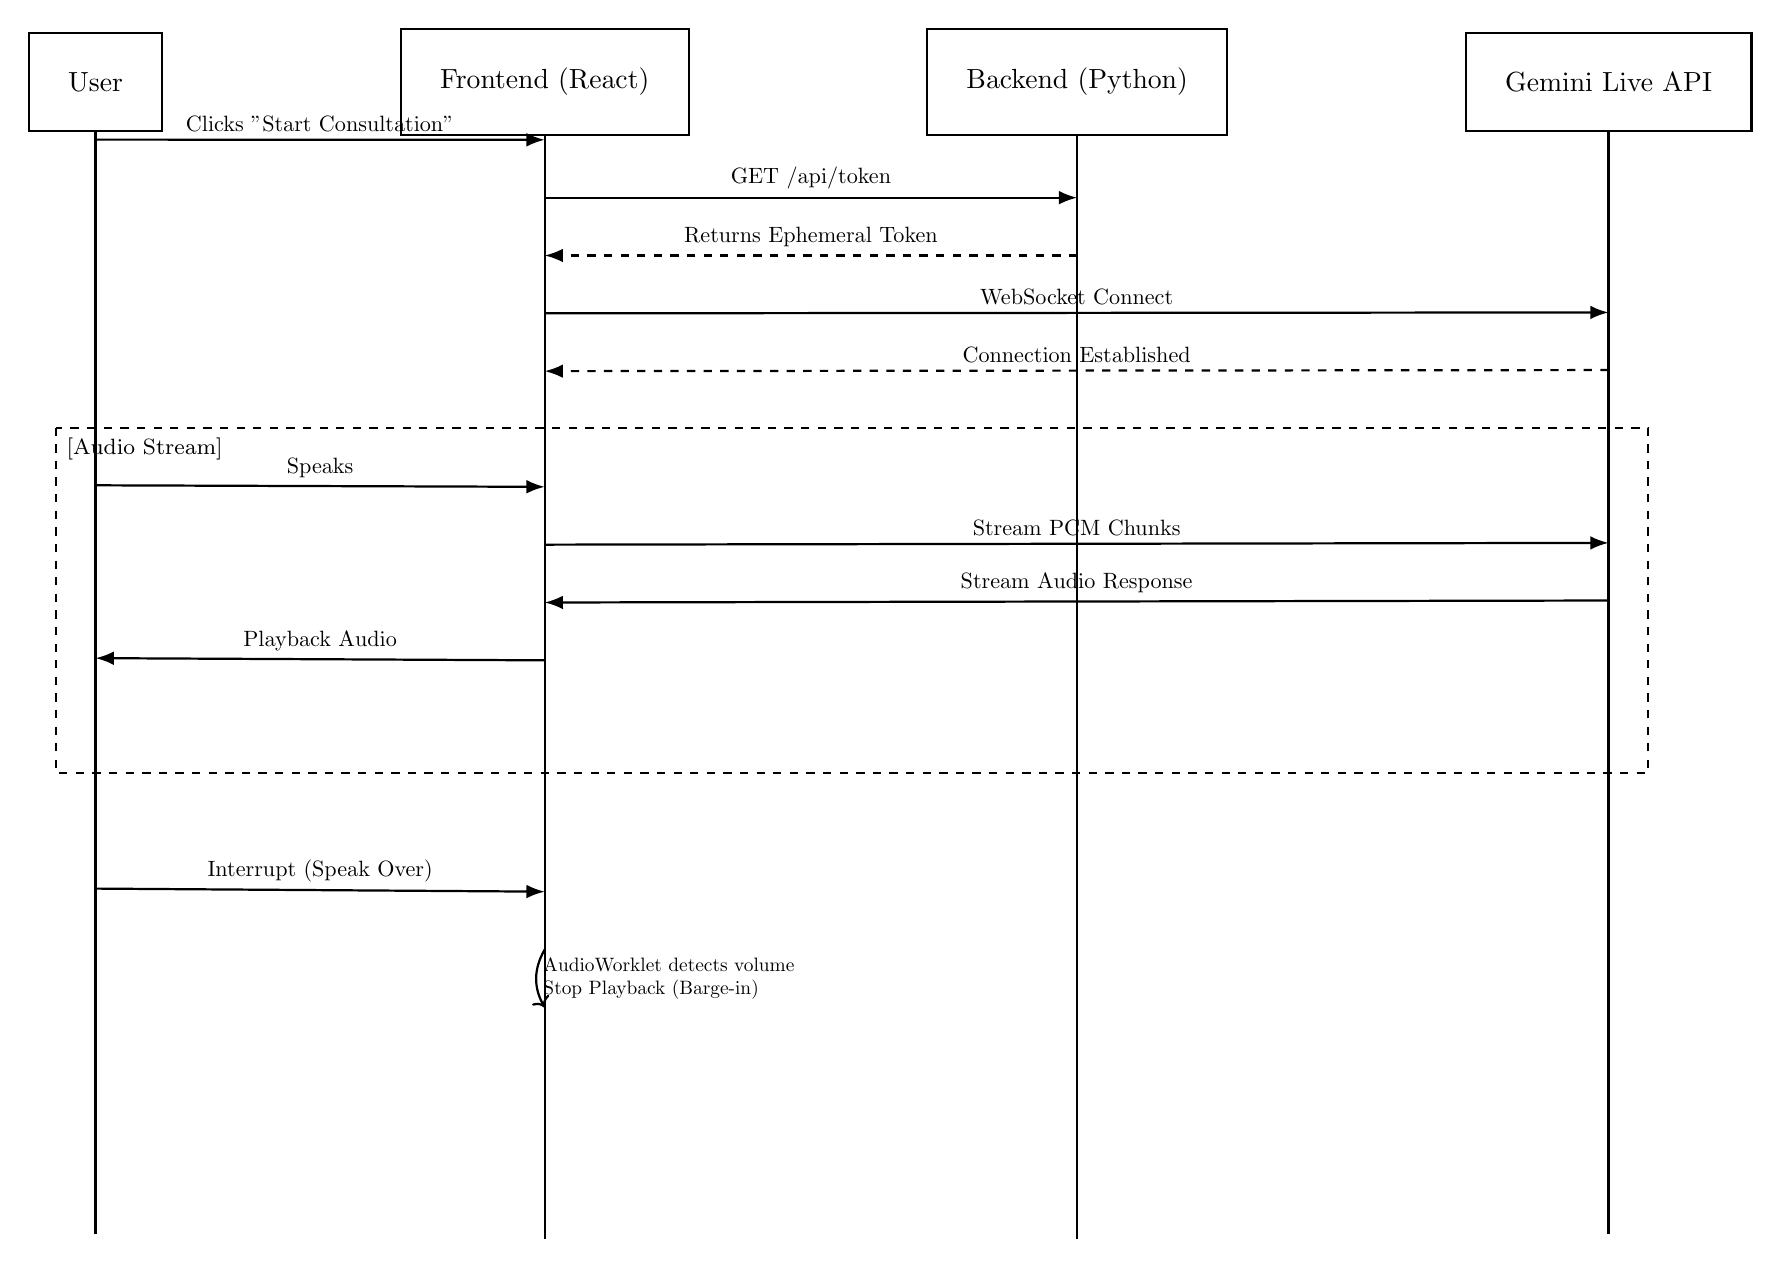
\begin{tikzpicture}[
        node distance=4cm,
        auto,
        thick,
        actor/.style={rectangle, draw, minimum size=1cm, inner sep=0.5cm, align=center},
        line/.style={draw, -Latex},
        dashed line/.style={draw, dashed, -Latex}
    ]
        % Actors
        \node[actor] (User) {User};
        \node[actor, right=3cm of User] (Client) {Frontend (React)};
        \node[actor, right=3cm of Client] (Server) {Backend (Python)};
        \node[actor, right=3cm of Server] (Gemini) {Gemini Live API};

        % Lifelines
        \coordinate (UserBottom) at ($(User.south)+(0,-14)$);
        \coordinate (ClientBottom) at ($(Client.south)+(0,-14)$);
        \coordinate (ServerBottom) at ($(Server.south)+(0,-14)$);
        \coordinate (GeminiBottom) at ($(Gemini.south)+(0,-14)$);

        \draw (User) -- (UserBottom);
        \draw (Client) -- (ClientBottom);
        \draw (Server) -- (ServerBottom);
        \draw (Gemini) -- (GeminiBottom);

        % Messages
        % Step 1
        \path (User) -- coordinate[pos=0.1] (y1) (UserBottom);
        \draw[line] ($(User)!0.05!(UserBottom)$) -- node[above, scale=0.8] {Clicks "Start Consultation"} ($(Client)!0.05!(ClientBottom)$);

        % Step 2
        \draw[line] ($(Client)!0.1!(ClientBottom)$) -- node[above, scale=0.8] {GET /api/token} ($(Server)!0.1!(ServerBottom)$);

        % Step 3
        \draw[dashed line] ($(Server)!0.15!(ServerBottom)$) -- node[above, scale=0.8] {Returns Ephemeral Token} ($(Client)!0.15!(ClientBottom)$);

        % Step 4
        \draw[line] ($(Client)!0.2!(ClientBottom)$) -- node[above, scale=0.8] {WebSocket Connect} ($(Gemini)!0.2!(GeminiBottom)$);

        % Step 5
        \draw[dashed line] ($(Gemini)!0.25!(GeminiBottom)$) -- node[above, scale=0.8] {Connection Established} ($(Client)!0.25!(ClientBottom)$);

        % Parallel Block
        \path ($(User)!0.3!(UserBottom)$) coordinate (parStart);
        \path ($(Gemini)!0.6!(GeminiBottom)$) coordinate (parEnd);
        \draw[dashed] ($(User)!0.3!(UserBottom) + (-0.5,0)$) rectangle ($(Gemini)!0.6!(GeminiBottom) + (0.5,0)$);
        \node[anchor=north west] at ($(User)!0.3!(UserBottom) + (-0.5,0)$) {\footnotesize [Audio Stream]};

        % Audio Stream Steps
        \draw[line] ($(User)!0.35!(UserBottom)$) -- node[above, scale=0.8] {Speaks} ($(Client)!0.35!(ClientBottom)$);
        \draw[line] ($(Client)!0.4!(ClientBottom)$) -- node[above, scale=0.8] {Stream PCM Chunks} ($(Gemini)!0.4!(GeminiBottom)$);
        \draw[line] ($(Gemini)!0.45!(GeminiBottom)$) -- node[above, scale=0.8] {Stream Audio Response} ($(Client)!0.45!(ClientBottom)$);
        \draw[line] ($(Client)!0.5!(ClientBottom)$) -- node[above, scale=0.8] {Playback Audio} ($(User)!0.5!(UserBottom)$);

        % Interrupt
        \draw[line] ($(User)!0.7!(UserBottom)$) -- node[above, scale=0.8] {Interrupt (Speak Over)} ($(Client)!0.7!(ClientBottom)$);
        \draw[->, bend right] ($(Client)!0.75!(ClientBottom)$) to node[right, scale=0.7, align=left] {AudioWorklet detects volume\\Stop Playback (Barge-in)} ($(Client)!0.8!(ClientBottom)$);

    \end{tikzpicture}
    }
    \caption{Voice Agent Interaction Flow}
\end{figure}

\subsection*{Architecture Flow}
\begin{enumerate}
    \item User clicks ``Start Consultation''.
    \item Client requests an Ephemeral Token from the Backend (GET /api/token).
    \item Backend returns a token valid for 30 minutes.
    \item Client establishes a direct WebSocket connection to Gemini Live API.
    \item Audio streaming begins (bidirectional).
    \item When the user interrupts (speaks over AI), the client detects volume and stops AI playback immediately (Barge-in).
\end{enumerate}

\section{WebSocket \& Data Flow}
The core interactions happen over a \textbf{Persistent WebSocket Connection} directly from the browser to Google's servers.

\begin{itemize}
    \item \textbf{Protocol}: The system uses the Gemini Live API directly via the \texttt{GoogleGenAI} client SDK in the browser.
    \item \textbf{Security}: The backend issues a short-lived ``ephemeral token''. This prevents exposing the master API key to the client while allowing the client to connect directly to Google.
    \item \textbf{Data Format}:
    \begin{itemize}
        \item \textbf{Input}: Raw PCM 16kHz audio (converted from Float32 to Int16) sent as base64 blobs in real-time.
        \item \textbf{Output}: Received audio chunks are decoded and queued for immediate playback.
    \end{itemize}
\end{itemize}

\section{Audio Optimizations \& ``Amazing Voice'' Features}

\subsection{Latency Reduction (Streaming)}
Instead of the traditional ``Record -- Stop -- Upload -- Transcribe -- Process'' loop, this system uses \textbf{Full Duplex Streaming}:
\begin{itemize}
    \item \textbf{Input Streaming}: Audio is captured via an \texttt{AudioWorklet} (\texttt{audio-processor.js}) and sent in small chunks ($\approx$ 2048 frames) instantly. This means the AI starts processing \textit{while} the user is still speaking.
    \item \textbf{Output Streaming}: Response audio is played chunk-by-chunk as it arrives using \textbf{Active Source Queueing}. The \texttt{nextStartTimeRef} logic ensures chunks play seamlessly without gaps or overlaps.
\end{itemize}

\subsection{``Barge-In'' / Interruption Logic}
To solve the ``not listening'' or ``rude AI'' problem, the system implements an \textbf{Interruption Mechanism}:
\begin{itemize}
    \item The \texttt{useGeminiLive} hook is designed to monitor audio levels.
    \item When the user speaks (detected via volume threshold), \texttt{cleanupAudio(true)} is triggered, which immediately:
    \begin{enumerate}
        \item Stops the current audio source nodes.
        \item Clears the playback queue.
        \item Effectively ``mutes'' the AI so it can listen to the user.
    \end{enumerate}
\end{itemize}

\subsection{Echo Cancellation \& ``Listening to Itself''}
\begin{itemize}
    \item \textbf{Echo Cancellation}: The system leverages the browser's native \texttt{MediaStream} processing (\texttt{echoCancellation: true} is standard in \texttt{getUserMedia}) to filter out the speaker output from the microphone input.
    \item \textbf{State Awareness}: The \texttt{isSpeaking} and \texttt{isListening} states manage the UI visualizer, giving the user visual feedback on when the AI is ``hearing'' them versus ``thinking''.
\end{itemize}

\subsection{Audio Worklet (Jitter-Free Processing)}
\begin{itemize}
    \item \textbf{Problem}: Main thread processes (UI updates, React renders) can block audio processing, causing pops/clicks.
    \item \textbf{Solution}: An \texttt{AudioWorklet} (\texttt{audio-processor.js}) is used to handle raw audio data in a separate thread. This ensures that audio capture is smooth and consistent even if the UI is busy rendering complex animations.
\end{itemize}

\section{Workflow Summary}
\begin{enumerate}
    \item \textbf{Connection}: Client fetches token $\rightarrow$ Initializes Audio Contexts $\rightarrow$ Connects to Gemini.
    \item \textbf{Assessment}: The AI follows a ``System Instruction'' (\texttt{LAWYER\_SYSTEM\_INSTRUCTION}) to guide the conversation.
    \item \textbf{Conclusion}: When the goal is met, the AI calls the \texttt{save\_session\_summary} tool.
    \item \textbf{Persistence}: The client intercepts this tool call, sends the data to the backend (\texttt{POST /api/sessions}), and then disconnects.
\end{enumerate}

\section{Technology Stack}
\begin{itemize}
    \item \textbf{Frontend}: React, TypeScript, Vite
    \item \textbf{Audio}: Web Audio API (AudioContext, AudioWorklet, AudioBufferSourceNode)
    \item \textbf{AI/Voice}: Google GenAI SDK (Gemini Live Multimodal)
    \item \textbf{Backend}: Python (aiohttp), storing sessions in JSON/Filesystem.
\end{itemize}

\end{document}
